\documentclass[12pt,twoside,a4paper]{article}
\usepackage{listings}
\usepackage{tcolorbox}
\usepackage{placeins}
\usepackage{hyperref}
\usepackage{float}
\newcommand{\lstfont}[1]{\color{#1}\scriptsize\ttfamily}

\lstset{
    language=[ANSI]C++,
    showstringspaces=false,
    backgroundcolor=\color{black!90},
    basicstyle=\lstfont{white},
    identifierstyle=\lstfont{white},
    keywordstyle=\lstfont{magenta!40},
    numberstyle=\lstfont{white},
    stringstyle=\lstfont{cyan},
    commentstyle=\lstfont{yellow!30},
    emph={
        cudaMalloc, cudaFree,
        __global__, __shared__, __device__, __host__,
        __syncthreads,
    },
    emphstyle={\lstfont{green!60!white}},
    breaklines=true
}


\title{GPU Computing\\
Exercise 2}
\author{
  Luis Wenzel\\
  Miro Joensuu\\
  Daniel Bayer\\
  Noah Schneider
}
\date{}

\begin{document}

\maketitle
\section{Presenting}
Willing to present:\\
3.1 Yes\\
3.2 Yes\\
3.3 Yes\\
3.4 Yes \\
\section{Global Memory - cudaMemcpy} 
\subsection{cudaMemcpy Task}

In this Task, the use of cudaMalloc(\&hmem, dat); and cudaMemcpy(hmem, dmem, dat, cudaMemcpyDeviceToDevice); was analyzed. That way we copy data from device to device. In the Graph \ref{fig:exc03_1_D2D} we can see, that a saturation of the coppying speed occurs on higher data transportation rates. In our Graph, we also show the other coppying speed of the other data. If you would like to take a look at our data, the data of the graphs is in folder (\url{exc03/Latex_File/data/analysis}).

\begin{figure}[H]
    \centering
    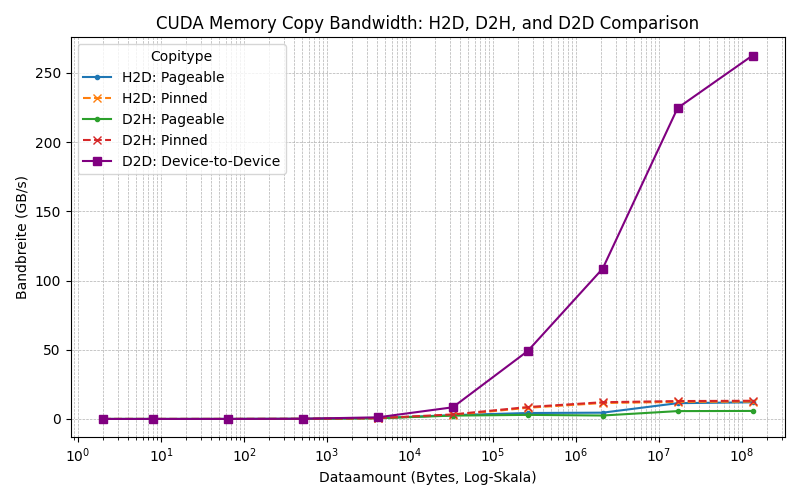
\includegraphics[width=1\textwidth]{pictures/exc03_1_D2D_together.png}
    \caption{Speed difference of Device to Device memory copy}
    \label{fig:exc03_1_D2D}
\end{figure}

\subsection{coalesced thread access}
In this exersise we copy data from device to device using a for loop and multiple threads accessing memory in a coalesced manner.
First we utilize only one threadblock and vary the number of threads. Using more threads, we expectedly increase the rate
at which we are able to copy data from global to global memory. The amount of parallelism increases with more threads.
The advantage is small at small data sizes but increases ever larger at larger datasizes as we have less overhead.
We reach peak transfer speeds with 1024 threads already quite early at 1MB with around 18 GB/s with 1024 threads,
after which the performance drops. Possibly this could have something to do with the size of the L2 cache of around
1MB, where with data larger than 1MB the threads have to deal with slower and multiple accesses to main memory.

\begin{figure}
    \centering
    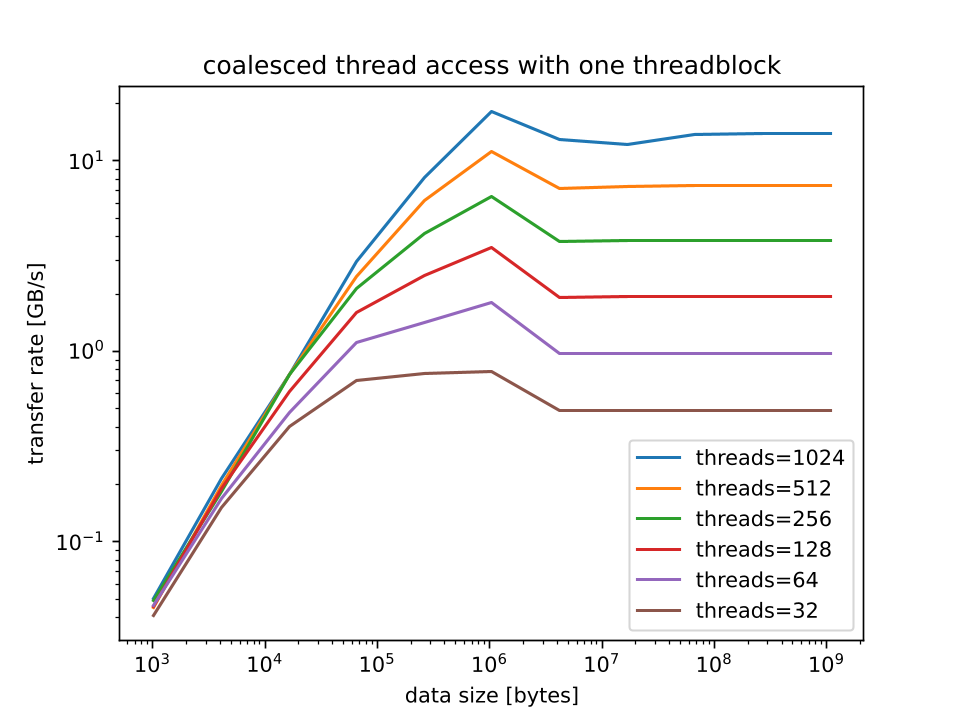
\includegraphics[scale=0.7]{pictures/coalesced_thread_access_a.png}
    \caption{exercise 2.2: 1 threadblock, different numbers of threads}
    \label{fig:2.2a}
\end{figure}

Next we varied the number of threadblocks for the peak-performing 1024 threads. Also here we can see the advantage
of more threadblocks emerge only at larger data sizes. Peak performance is reached with the maximum 32 threadblocks at
a data size of 67MB with 212 GB/s, close to the cudaMemcpy bandwidth. More parallelism in this case also means higher transfer speeds.
As with varying the number of threads, the performance is best at a few MB but drops slightly when reaching even larger data sizes around 1GB.
Again this could have to do with the size of the L2 cache. The optimal performance was reached with the maximum number of threads (1024) and
threadblocks (32).

\begin{figure}
    \centering
    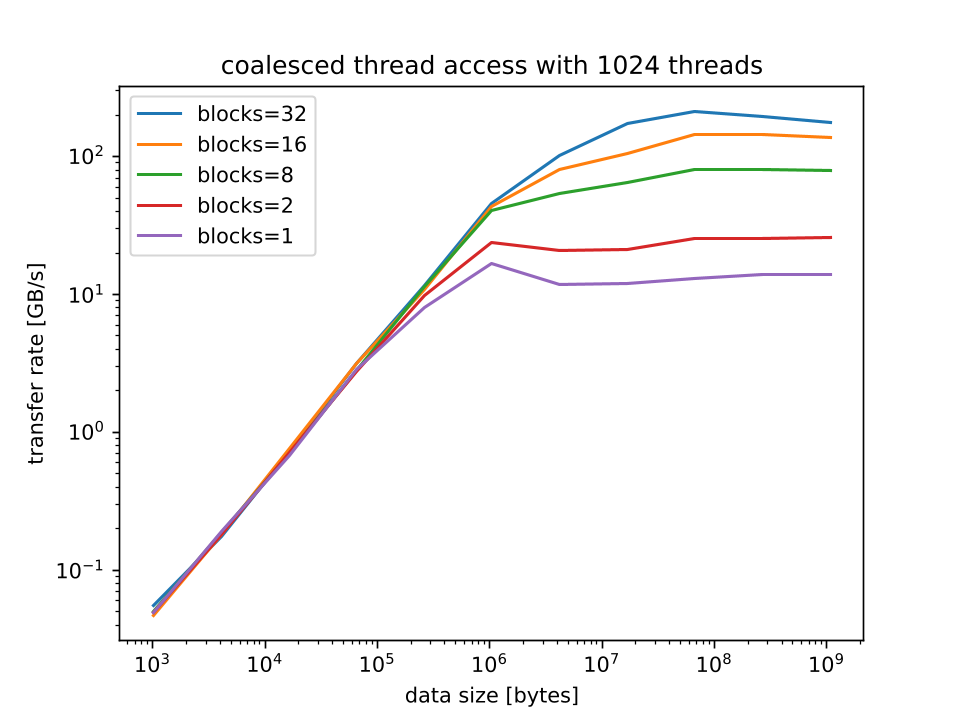
\includegraphics[scale=0.7]{pictures/coalesced_thread_access_b.png}
    \caption{exercise 2.2: 1024 threads, different numbers of blocks}
    \label{fig:2.2b}
\end{figure}	

\subsection{thread access with stride}
Now instead of using coalesced thread access, where each thread accesses a contiguous element in memory,
we use a stride. This leads to more memory transactions as more cache lines have to be pulled from memory to
satisfy the memory requests coming from one threadwarp. It also leads to an underutilized cache as more cache
lines have to be pulled. This problem should get worse with an increasing stride. In our results, however, while
the performance drops we do not see an exponential decrease in the performance as expected. In fact, at a stride of
128 the performance jumps back up and above our baseline coalesced result. We presume that this could either have to do
with our small data sizes of only 64kB (16 threadblocks x 1024 threads x 4 bytes per thread), where launch
overhead still dominates above proper cache utilization. Although, as the data we want to transfer should exceed the maximum
L1 cache capacity of 48kB, underutilizing cache should start to become a problem. Another possible explanation is, of course,
a mistake in the code. This is shown in figure \ref{fig:2.3}.


\begin{figure}
    \centering
    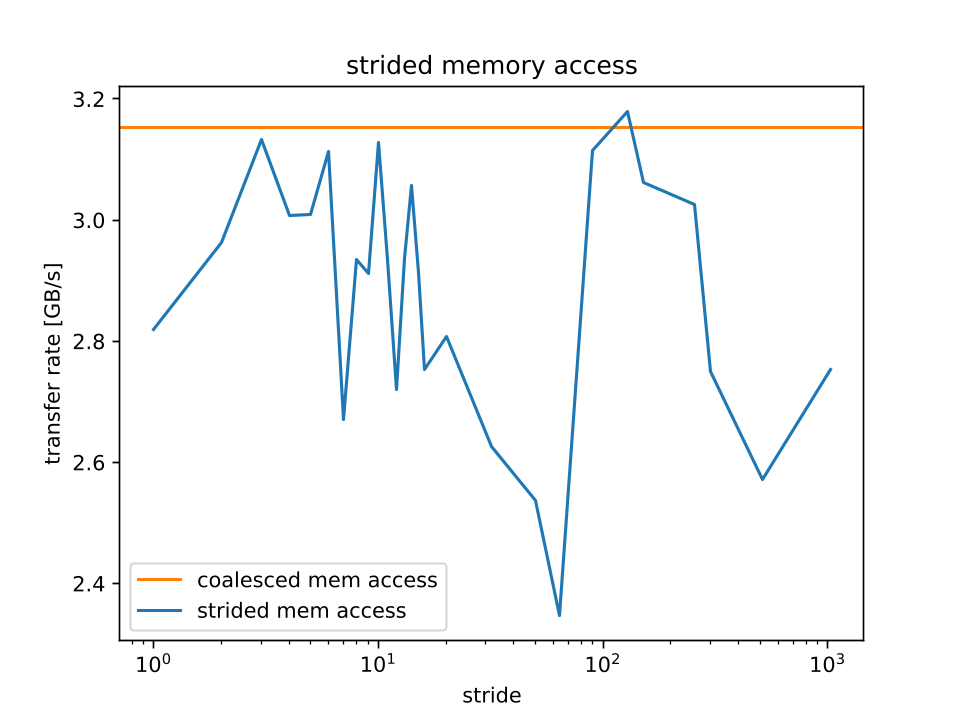
\includegraphics[scale=0.7]{pictures/strided_thread_access.png}
    \caption{exercise 3.3, thread access with stride}
    \label{fig:2.3}
\end{figure}

<<<<<<< HEAD
\subsection{thread access with offset}
Using an offset instead of a stride should also lead to underutilization of the cache, but not
in a way that is as dramatic as using a stride. Only sometimes could the boundary of a cache line be crossed and an
extra cache line would have to be fetched from memory. E.g. with a warp size of 32 and 4 bytes per element, one
warp would pull 1 full cache line of 128 bytes. With an offset of 1, this would no longer be the case, an extra cache line
would have to be pulled from memory. Again, our results are mixed. We see a large drop off in memory for small offsets, but this recovers
around an offset of 12 back to the value of the coalesced memory access speed. Again, this could be due to a too small data size used here, or
due to a coding mistake. This is shown in figure \ref{fig:2.4}.

\begin{figure}
    \centering
    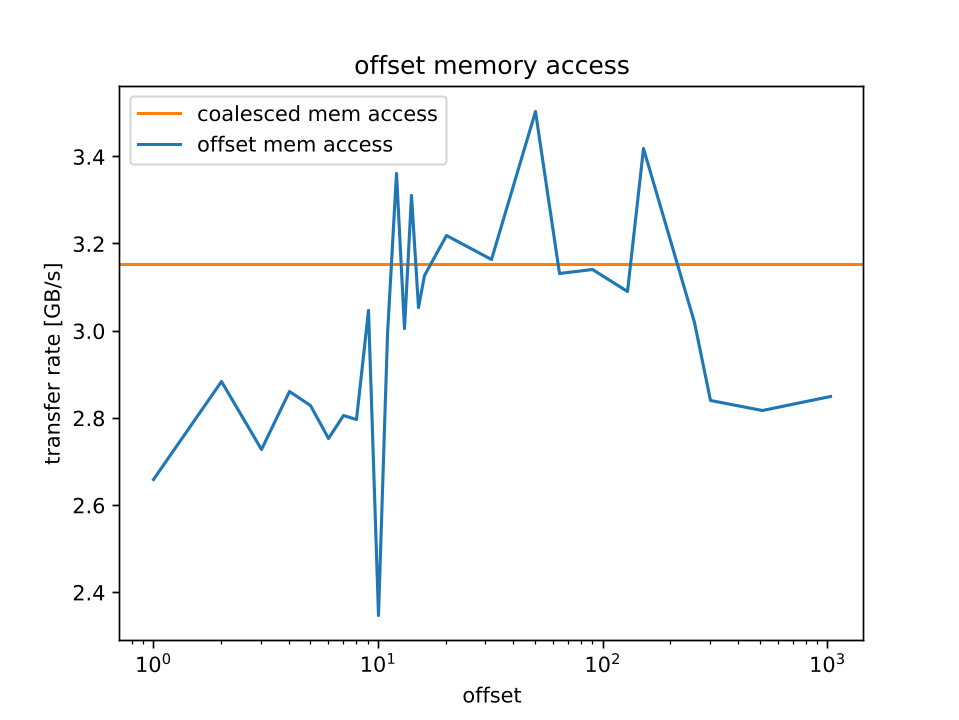
\includegraphics[scale=0.7]{pictures/offset_thread_access.png}
    \caption{exercise 3.4, thread access with offset}
    \label{fig:2.4}
\end{figure}
=======
\subsection{Global Memory -thread access with offset}
>>>>>>> 792f72f665a582f24594403cf1deafa1b2bb9d66

\FloatBarrier


\end{document}
